\documentclass[a4paper,9pt,twocolumn]{jsarticle}
\usepackage{eshouroku}
\usepackage[dvipdfmx]{graphicx}
\usepackage{amsmath}
\usepackage{url}
\usepackage{here}
\usepackage{booktabs}
\usepackage{remreset}
\usepackage{pdfpages}
\usepackage{comment}
\usepackage{subfigure}
\usepackage{amsmath}
\renewcommand{\baselinestretch}{0.9}

\renewcommand{\subfigtopskip}{5pt}	% 図の上の隙間。上図の副題と下図の間。
\renewcommand{\subfigbottomskip}{0pt} % 図の下の隙間。副題と本題の間。
\renewcommand{\subfigcapskip}{-6pt}	% 図と副題の間
\renewcommand{\subcapsize}{\scriptsize} % 副題の文字の大きさ


\makeatletter
	\renewcommand{\theequation}{% 式番号の付け方
	\thesection\arabic{equation}}
	\@addtoreset{equation}{section}

	\renewcommand{\thefigure}{% 図番号の付け方
	\thesection\arabic{figure}}
	\@addtoreset{figure}{section}

	\renewcommand{\thetable}{% 表番号の付け方
	\thesection\arabic{table}}
	\@addtoreset{table}{section}
\makeatother
%\numberwithin{equation}{section}
%\numberwithin{table}{section}
%\numberwithin{figure}{section}


% 数式(演算子など)のスペースを詰める
% =,→ 間の余白
\thickmuskip=1.0\thickmuskip
% +,- 間の余白
\medmuskip=0.8\medmuskip
% … などの装飾記号の余白
\thinmuskip=0.8\thinmuskip
% 行列を詰める
\arraycolsep=0.3\arraycolsep
% 数式の上下のスペースの変更
\AtBeginDocument{
  \abovedisplayskip     =0.5\abovedisplayskip
  \abovedisplayshortskip=0.5\abovedisplayshortskip
  \belowdisplayskip     =0.5\belowdisplayskip
  \belowdisplayshortskip=0.5\belowdisplayshortskip}


\boldmaintrue% 主文を太字にするモード(指導教員添削時はこちら)
%\boldmainfalse% 主文を普通文字にするモード(抄録印刷時はこちら)
\graphicspath{{./figs}}
\begin{document}
\twocolumn[
 \講演番号{B-XX}% 必要ない場合には書かない
 \日本語タイトル{\huge}{神経免疫相互作用に着想を得た\\マルチエージェントシステム型ニューラルネットワークの提案}
 \英語タイトル{\large}{Proposal of Neural Network composed of Multi-Agent System Inspired by Nervous-Immune Interaction}
 \筆者一名{5335}{柚木開登}

 \指導教員一名{山本哲也}
 %\指導教員二名{東京花子}{京都紀夫}
 %\指導教員なし
]

%\addcontentsline{toc}{section}{\refname}% 追加

\graphicspath{{./figs/}} % 図が特定のフォルダにある場合には設定

\section{本研究の意義・目的}
\begin{comment}
本来的に大規模な計算資源を必要とするニューラルネットワークが
今日, あらゆる産業へ導入されるに至ったのは, クラウドコンピューティングの貢献がある.
一方で, 同市場拡大に伴って
プラットフォーマによる市場寡占, データセンターでの電力消費, データプライバシーの課題が表面化した.
こうしたクラウドの課題克服に向けて, 
データを集約せずにネットワークの端点(エッジ)で処理するエッジコンピューティングが注目
されている.
\end{comment}
エッジコンピューティングでの機械学習手法として連合学習(Federareted Lerning)が提案されている.
連合学習では, 学習データを集約せずネットワーク中の各ノードで学習し, 
その結果得たパラメータ差分のみを通信し, 平均化することで
大規模な学習済みモデルを構築するため, プライバシーを含んだ学習データは各ノード内に保護される.
機械学習への期待と世界的な個人情報保護の動きの高まりから, 
将来的に連合学習は情報社会において重要な位置を占めることが予測される.

一方, 連合学習の実用化に際しては, 
従来, データセンターで動いていたモデルを計算資源に乏しいエッジ環境に投入する必要があることから
少なくとも以下2点の課題が考えられる.
1つ目は学習パラメータ削減によるモデルの軽量化, 
2つ目は, エッジ環境内の不均一計算資源の利用
である.
両者を満たしたモデルを構築できれば, 
大規模なニューラルネットワークのエッジ環境への投入を可能にし, 
かつ環境内の計算資源の利用率を最大化することが期待できるが,  
両者を満たしたモデルに関する研究は著者の知る限り存在しない.

そこで本研究では, 将来的に導入が予測されるエッジコンピューティングアーキテクチャ及び, 
それに対応した機械学習手法である連合学習に向けて, 
自律分散性を持ったニューラルネットワークのパラメータ削減を提案する(\wfig{ThisModel}).
提案にあたっては, 生体の脳における自律分散的なパラメータ削減である
グリア細胞による神経回路の刈り込みに着目し, 
神経免疫相互作用に基づくニューロンとグリアの相互調節機構をマルチエージェントシステムとして実装した.
\begin{figure}[H]
  \centering
  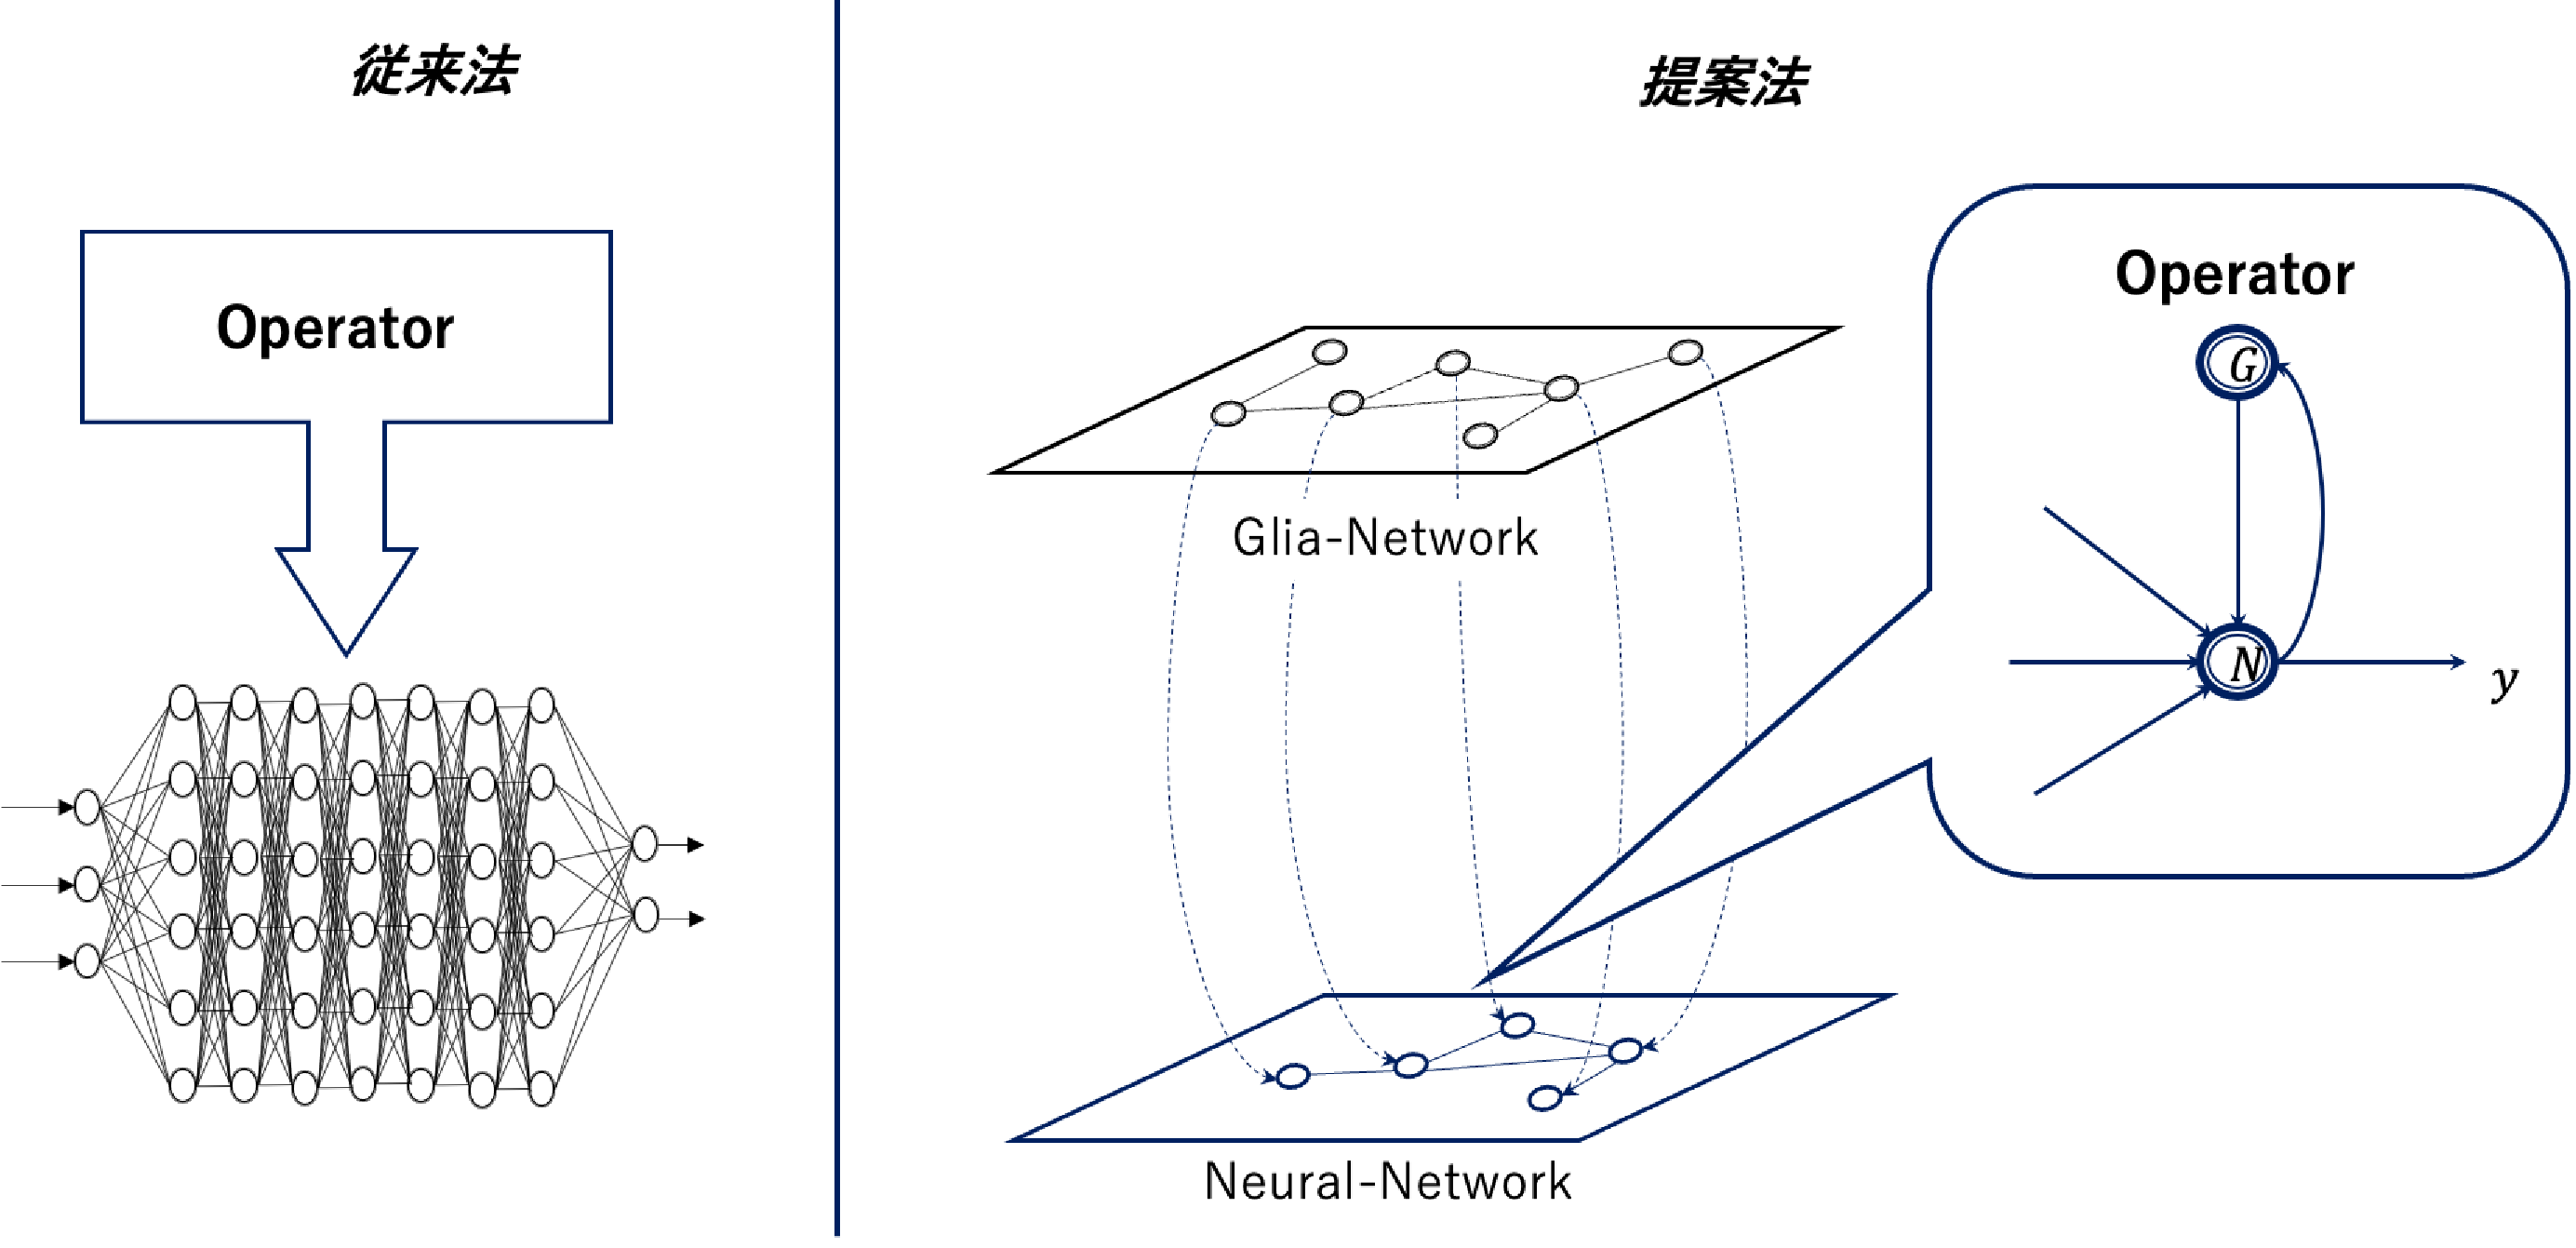
\includegraphics[width=8cm]{ThisModel.pdf}
  \label{fig:ThisModel}
\end{figure}
\vspace{-4zh}
\section{提案モデル}
\subsection{複数のエージェントシステムによるニューラルネットワーク}
本提案は, 細胞間ネットワークとしての生体システムの模倣及び, 
自律分散性の保証といった観点からマルチエージェントシステムとして解釈・実装している.  
以下, 投入するエージェントについて説明する.
  \subsubsection*{●Neuro-Agent}
  神経細胞をモデル化したエージェントであり, 情報の受容, 処理, 
  転送などを担当する.
  それぞれのNeuro-Agentは, 情報を受け取るための複数の入力$x_i$ $\;(i= 1, 2, 3, \cdots m)$と, 
  内部変数$b$を持ち, 
  これを処理して別のNeuro-Agentに情報を送信するための出力$y$を生成する.
  この時の内部処理は, \weq{Neuro-Agent}に示す通り, 標準的な人工ニューロンと同等である.
  \
  \begin{align}
    y=\phi(\sum_{i=1}^m x_i+b)
    \label{eq:Neuro-Agent}
  \end{align}
  \subsubsection*{●Synapse-Agent}
  神経回路における接触構造であるシナプスをモデル化したエージェントであり, 
  Neuro-Agent間の情報の伝達を担当する.
  それぞれのSynapse-Agentは, 入力$u$を受け取り, それを変換した値$v$を出力する(\weq{Synapse-Agent}). 
  この出力は別のNeuro-Agentの入力として使用される.
  \begin{align}
    v=weight\cdot u
 \label{eq:Synapse-Agent}   
  \end{align}
  ここで, 式中の$weight$は, そのSynapse-Agentの重みを示し, 
  主にこれを誤差逆伝播法を用いて更新することで, ニューラルネットワークが学習される.
  \subsubsection*{●Glia-Agent}神経細胞の補助細胞であるグリア細胞(Glia-Cell)の機能を模倣したエージェント。
  Glia-Agentは, Neuro-AgentとSynapse-Agentによって構成されるニューラルネットワークに対して,
  シナプスの刈り込みを行い, パラメータ削減による学習の効率化・高速化を試みる. 

\subsection{神経免疫相互作用に基づく相互調節モデル}
次に, 具体的にGlia-AgentがNeuro-Agentに対して行う刈り込み命令の発出, 及び
Neuro-AgentからGlia-Agentへのフィードバックによる刈り込みの制御について説明する.

Glia-AgentとNeuro-Agentは\wfig{NeuroGlia}に示すように, 1:1で接続され相互に調節を行う.
\begin{figure}[H]
  \centering
  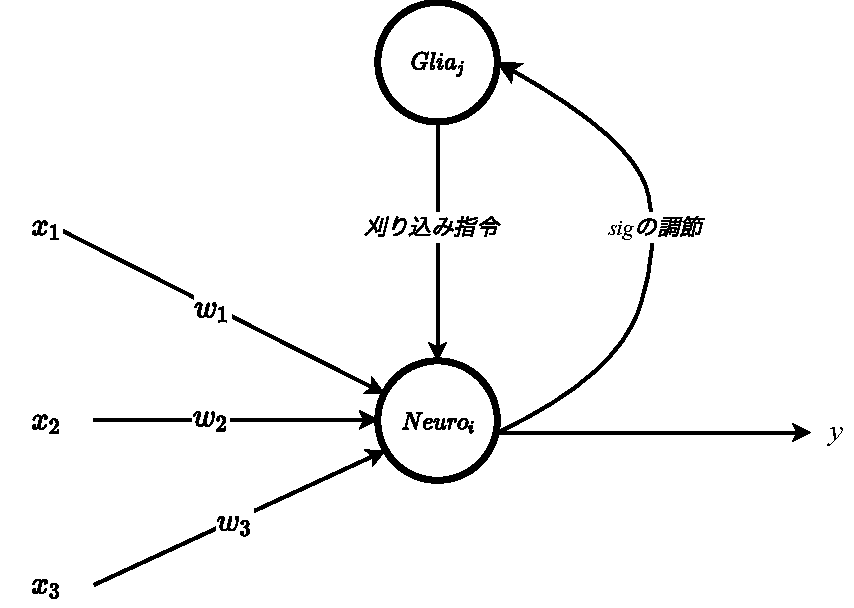
\includegraphics[width=7cm]{NeuroGlia.pdf}  
  \label{fig:NeuroGlia}
  \caption{Neuro-Glia相互調節機構}
\end{figure}
\vspace{-2zh}
\subsubsection*{Glia-AgentからNeuro-Agentへの作用:刈り込み命令の発出}
シナプスの刈り込み命令はGlia-Agentの内部変数$sig$
を閾値に用いて確率的に実行される.
Neuro-Agentは刈り込み命令を受け取ると, 自身に接続された最も重みが0に近いSynapse-Agentを
削除する.
\subsubsection*{Neuro-AgentからGlia-Agentへの作用:$sig$の調節}
逆に, Neuro-Agentは自身の活動頻度$freq$を用いて, Glia-Agentの内部変数$sig$を更新する.
この更新式は, \weq{sig}に示す通りである.
\begin{align}
  sig\leftarrow sig-&\cfrac{2}{1-6\ln(3)\exp(Neuro.freq-0.01)}-1
  \label{eq:sig}
\end{align}
\weq{sig}が示す等に, Neuro-Agentは自身の活動頻度$freq$が高ければ, $sig$を上げることで刈り込まれにくく, 
逆に$freq$が0に近いほど$sig$を下げ刈り込み命令の発出を容易するようにフィードバックを行う.
\subsection{グリアネットワーク}
実際の脳ではグリア細胞は単体で
刈り込みを行っているのではなく, 
グリアアセンブリと呼ばれるグリア細胞同士のネットワークを介して, 
協調し全体としての利益に資する行動をとっているものと見られる.

本モデルはグリアアセンブリの模倣として$Glia-Agent$同士のネットワークである
グリアネットワークを定義した.
グリアネットワークは, 抑制信号$sig$を他の$Glia-Agent$に伝播する.
これにより, 時空間的に局所的な刈り込みを抑制し, ネットワークの破綻を防ぐ役割がある.

抑制信号は, グリアネットワーク上の伝播距離(ホップ数)に応じて減衰定数$A$だけ減衰していく.
なお, 複数の距離が与えられた場合, 最も近い$Glia-Agent$の影響を優先する.
例えば, \wfig{GliaNetworks}の$g_2$の場合, 
$g_0\rightarrow g_1\rightarrow g_2$と$g_0\rightarrow g_2$の経路では後者の経路のみを考えることになる.
\begin{figure}[H]
  \centering
  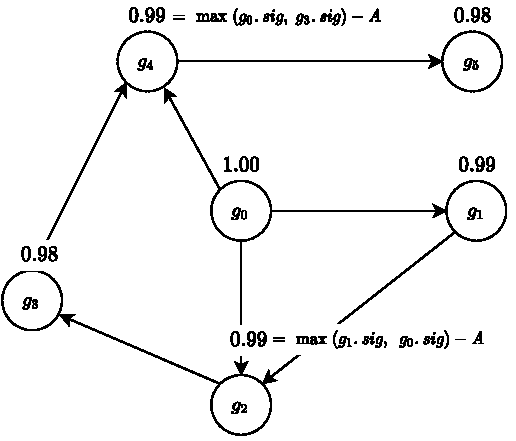
\includegraphics[width=4cm]{GliaNetworks.pdf}
  \caption{グリアネットワークでの抑制信号の伝達}
  \label{fig:GliaNetworks}
\end{figure}
\vspace{-3zh}
\section{計算機実験}
学習タスクとして6bitの入力の上位3bitのいずれかに1が入っているかどうか
の判別を行った出力値は結果が真である確率である. 
その他のパラメータは以下に示す通りである(\wtab{param}).
\begin{table}[H]
  \caption{パラメータ一覧}
  \label{tab:param}
  \centering
   \begin{tabular}{ll}
    \toprule
      パラメータ&値\\\midrule\midrule
      学習率$\eta$&$0.5$\\
      エポック数$Epocs$&$100$\\
      ミニバッチサイズ$miniBatchSize$&$100$\\
      初期ニューロン数$Neurons$&$31$\\
      初期グリア数$Glias$&$31$\\
      初期シナプス数$Mill$&$182$\\
      減衰率$A$&0.01\\
      入力サイズ$Inputs$&$6$\\
      出力サイズ$Outputs$&$1$\\
    \bottomrule
   \end{tabular}
 \end{table}
計算機実験の結果を\wfig{SynapseNum},\wfig{LearningCurve}に示す.
刈り込みを行った結果, 最終的なシナプス数は78に推移した.よって, 削減割合は
57%であり, また, \wfig{LearningCurve}より刈り込みによる精度悪化は認められないため, 
不要なシナプスの剪定が適切に行われたと評価できる.
\begin{figure}[H]
  \centering
  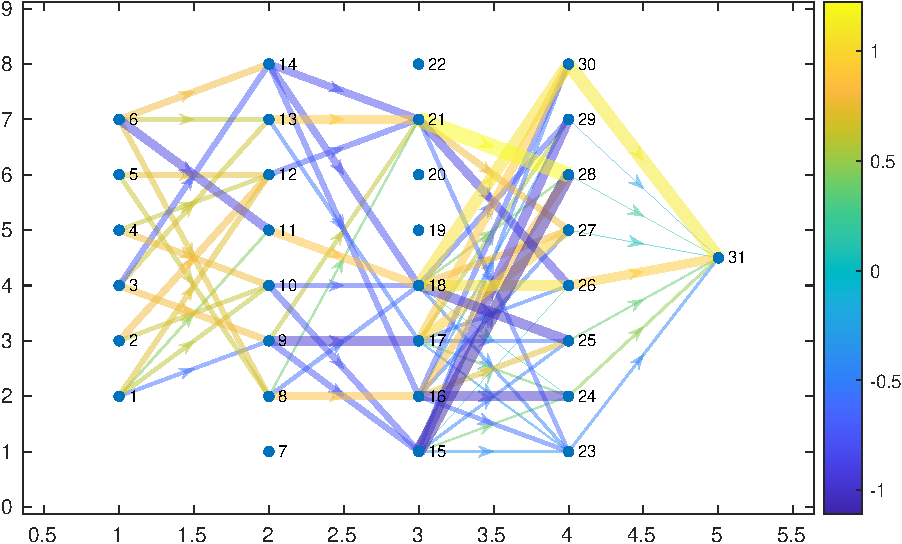
\includegraphics[width=8cm]{Graph-crop.pdf} 
  \caption{刈り込み後のネットワーク}
  \label{fig:Graph}
\end{figure}
\vspace{-2zh}
\begin{figure}[H]
  \centering
  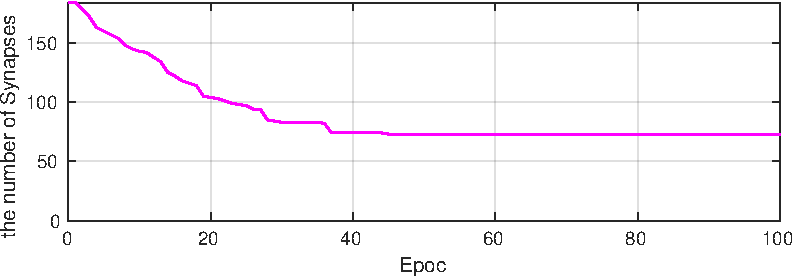
\includegraphics[width=8cm]{SynapseNum-crop.pdf} 
  \caption{シナプス量の変化}
  \label{fig:SynapseNum}
\end{figure}
\vspace{-2zh}
\begin{figure}[H]
  \centering
  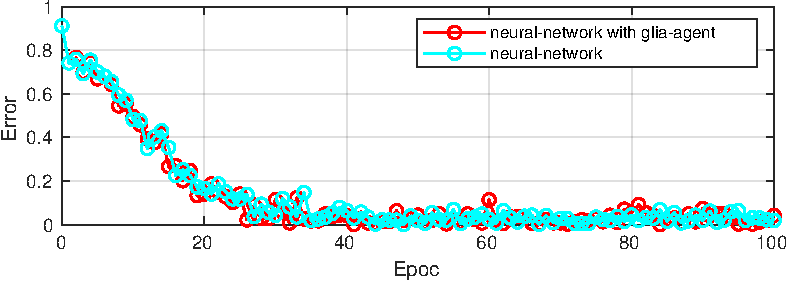
\includegraphics[width=8cm]{LearningCurve-crop.pdf} 
  \caption{学習曲線}
  \label{fig:LearningCurve}
\end{figure}
 
\section{結論}
グリア細胞に着想を得た監視エージェントを導入することによって
全体の管理者のいないMASに対応した
ニューラルネットワークの学習パラメータの削減を行うことができた.
このパラメータの削減にあたっては, 学習精度の悪化が認められなかったことから, 
刈り込みが適切に行われたものと評価できる
一方で, グリアネットワークの構造依存性や
MASに特有な問題(合意制御, 環境認識), あるいは畳み込みのMAS化など
実用化にあたっては
さらなる発展が必要である.
 \begin{thebibliography}{99}
  \bibitem{Neuron-Glia} 	
野村靖幸,北海道大学,神経免疫相関とくにニューロン・グリア相互作用機構に関する分子薬理学的研究, \url{https://kaken.nii.ac.jp/ja/grant/KAKENHI-PROJECT-06454595/}
  \bibitem{Tensorizing}
  Novikov, Alexander, et al. "Tensorizing neural networks." Advances in neural information processing systems 28 (2015).
  \bibitem{次数重み付き平均法}
  原田和明, 右田剛史, and 高橋規一.``ニューラルネットワークの分散学習における新たな合意重み決定法.'' IEICE Conferences Archives. The Institute of Electronics, Information and Communication Engineers, 2019.
\end{thebibliography}
 \end{document}
